%%%%%%%%%%%%%%%%%%%%%%%%%%%%%%%%%%%%%%%%%%%%%%%%%%%%%%%%%%%%%%%%%%%%%%%%%%%%%%%%%%%%%%%%%%%%%%%%
%
% CS576 Written Question Template
%
% Acknowledgements:
% The original code is written by Prof. James Tompkin (james_tompkin@brown.edu).
% The second version is revised by Prof. Min H. Kim (minhkim@kaist.ac.kr).
%
% This is a LaTeX document. LaTeX is a markup language for producing
% documents. Your task is to fill out this document, then to compile
% it into a PDF document.
%
%
% TO COMPILE:
% > pdflatex thisfile.tex
%
% If you do not have LaTeX and need a LaTeX distribution:
% - Personal laptops (all common OS): www.latex-project.org/get/
% - We recommend latex compiler miktex (https://miktex.org/) for windows,
%   macTex (http://www.tug.org/mactex/) for macOS users.
%   And TeXstudio(http://www.texstudio.org/) for latex editor.
%   You should install both compiler and editor for editing latex.
%   The another option is Overleaf (https://www.overleaf.com/) which is
%   an online latex editor.
%
% If you need help with LaTeX, please come to office hours.
% Or, there is plenty of help online:
% https://en.wikibooks.org/wiki/LaTeX
%
% Good luck!
% Min and the CS576 staff
%
%%%%%%%%%%%%%%%%%%%%%%%%%%%%%%%%%%%%%%%%%%%%%%%%%%%%%%%%%%%%%%%%%%%%%%%%%%%%%%%%%%%%%%%%%%%%%%%%
%
% How to include two graphics on the same line:
%
% \includegraphics[\width=0.49\linewidth]{yourgraphic1.png}
% \includegraphics[\width=0.49\linewidth]{yourgraphic2.png}
%
% How to include equations:
%
% \begin{equation}
% y = mx+c
% \end{equation}
%
%%%%%%%%%%%%%%%%%%%%%%%%%%%%%%%%%%%%%%%%%%%%%%%%%%%%%%%%%%%%%%%%%%%%%%%%%%%%%%%%%%%%%%%%%%%%%%%%

\documentclass[11pt]{article}

\usepackage[english]{babel}
\usepackage[utf8]{inputenc}
\usepackage[colorlinks = true,
            linkcolor = blue,
            urlcolor  = blue]{hyperref}
\usepackage[a4paper,margin=1.5in]{geometry}
\usepackage{stackengine,graphicx}
\usepackage{fancyhdr}
\setlength{\headheight}{15pt}
\usepackage{microtype}
\usepackage{times}
\usepackage{booktabs}

% From https://ctan.org/pkg/matlab-prettifier
\usepackage[numbered,framed]{matlab-prettifier}

\frenchspacing
\setlength{\parindent}{0cm} % Default is 15pt.
\setlength{\parskip}{0.3cm plus1mm minus1mm}

\pagestyle{fancy}
\fancyhf{}
\lhead{Homework Writeup}
\rhead{CS576}
\rfoot{\thepage}

\date{}

\title{\vspace{-1cm}Homework 2 Writeup}


\begin{document}
\maketitle
\vspace{-3cm}
\thispagestyle{fancy}

\section*{Instructions}
\begin{itemize}
  \item Describe any interesting decisions you made to write your algorithm.
  \item Show and discuss the results of your algorithm.
  \item Feel free to include code snippets, images, and equations.
  \item There is no page limit.

\end{itemize}


\section*{Interesting Implementation Detail}


My code snippet highlights an interesting point.


\lstset{numbers = left, numbersep=5pt, breaklines=true}
\begin{lstlisting}[language=python, caption = {HOG Feature extraction}]
    if feature == 'HoG':
        # HoG parameters
        win_size = (32, 32)
        block_size = (32, 32)
        block_stride = (16, 16)
        cell_size = (16, 16)
        nbins = 9
        deriv_aperture = 1
        win_sigma = 4
        histogram_norm_type = 0
        l2_hys_threshold = 2.0000000000000001e-01
        gamma_correction = 0
        nlevels = 64


        # Your code here. You should also change the return value.

        # make HOG descriptor model with given parameter
        hog = cv2.HOGDescriptor(win_size, block_size, block_stride, cell_size, nbins, deriv_aperture, win_sigma, histogram_norm_type, l2_hys_threshold, gamma_correction, nlevels)

        m = img.shape[0]
        n = img.shape[1]

        all_f = []

        # divide original image with 16 X 16 grid and make subimages, so find HoG descriptor by grouped 4 cell (32 X 32) and 16 X 16 stride
        for i in range(int(m / 16) - 1):
            for j in range(int(n / 16) - 1):
                x = i * 16
                y = j * 16
                h = hog.compute(img[x:x+32, y:y+32])
                all_f.append(np.reshape(h, (1, 36)))

        # combine Hog desciptor from sub images
        all_f = np.concatenate(all_f, 0)
        return all_f
\end{lstlisting}

\lstset{numbers = left, numbersep=5pt, breaklines=true}
\begin{lstlisting}[language=python, caption = {SIFT Feature extraction}]
        m = img.shape[0]
        n = img.shape[1]

        all_f = []
        gray = cv2.cvtColor(img, cv2.COLOR_BGR2GRAY)
        sift = cv2.xfeatures2d.SIFT_create()

        # divide original image with 20 X 20 grid and make subimages, so find SIFT descriptor by 20 X 20 sub images.
        for i in range(int(m / 20)):
            for j in range(int(n / 20)):
                x = i * 20
                y = j * 20
                kp, des = sift.detectAndCompute(gray[x:x+20, y:y+20], None)
                if len(kp) != 0:
                    all_f.append(des)
                    
        #If sift is not detected, exception handling is done.
        if len(all_f) != 0:
            all_f = np.concatenate(all_f, 0)
        else:
            all_f = None

        return all_f
\end{lstlisting}

In both HOG and SIFT, because there was a difference between applying the descriptor to the entire image at one time and dividing whole image and directly into the sub-image, so  I chose the latter. The details of the algorithm are annotated in the above code block.

\lstset{numbers = left, numbersep=5pt, breaklines=true}
\begin{lstlisting}[language=python, caption = {K-means Clustering}]
    # Your code here. You should also change the return value.
    np.random.seed(0)
    n = all_features.shape[0]
    f_n = all_features.shape[1]
    center = np.zeros((vocab_size, f_n))

    # I choose start points as random sample of all_feature
    idx = np.random.choice(n, vocab_size, replace=False)
    for i in range(vocab_size):
        center[i, :] = all_features[idx[i], :]

    # In the worst case, iterations up to max_iter
    for k in range(max_iter):

        # back-up of previous center points, because of compare of epsilon
        prev_center = np.copy(center)

        # get distance between center points and feature points and labeling of feature using np.argmin
        d = pdist(all_features, center)
        lab = np.argmin(d, axis=1)

        # For empty cluster cases, align the points in the order that is farthest from the that point's center
        mind = np.min(d, axis=1)
        sort_arg = np.argsort(mind * -1)

        # Use the labels to update the center points to the average of the points in the cluster.
        center = np.zeros((vocab_size, f_n))
        num = np.zeros(vocab_size)
        for i in range(n):
            center[lab[i], :] = center[lab[i], :] + all_features[i, :]
            num[lab[i]] += 1

        # In empty case, the empty cluster is divided by 0. Therefore, to prevent this, the point that is farthest from the center is adopted as a new center.
        id = 0
        for i in range(vocab_size):
            if num[i] == 0:
                center[i, :] = all_features[sort_arg[id], :]
                id += 1
            else:
                center[i, :] = center[i, :] / num[i]

        # The ending condition is checked by comparing the previous center point with the current point.
        d2 = pdist(prev_center, center)
        maxe = 0
        for i in range(vocab_size):
            if maxe < d2[i, i]:
                maxe = d2[i, i]

        if maxe < epsilon:
            break

    return center
\end{lstlisting}
 
The special things I used to implement K-means are ,first, I choose start points as random sample of all feature and second, in the empty cluster case, to prevent this, the point that is farthest from the center is adopted as a new center. The details of the algorithm are annotated in the above code block.


\lstset{numbers = left, numbersep=5pt, breaklines=true}
\begin{lstlisting}[language=python, caption = {PCA}]
    n = vocab.shape[0]
    f_n = vocab.shape[1]
    f = np.copy(vocab)

    # subtract average of each coordinate
    for i in range(f_n):
        f[:,i] = f[:,i] - np.average(f[:,i])

    # make covariance matrix using matrix multiplication (X - X_bar)^T * (X - X_bar) / N
    cov = np.matmul(np.transpose(f), f)
    cov = cov / n

    # The eigenvector corresponding to dominate eigenvalue are equal to the first,second,.. column vector of V when a singular value decomposition.
    u, s, vh = np.linalg.svd(cov, full_matrices=True)
    v = np.transpose(vh)

    # In order to obtain the principal component of each voca, I compute the inner product feature vector with eigenvector.
    pca_f = np.zeros((n, feat_num))
    for i in range(feat_num):
        pca_f[:,i] = np.reshape(np.matmul(f, np.reshape(v[:,i], (-1,1))), -1)

    return pca_f
\end{lstlisting}

First, I subtract average of each coordinate from vocabulary vectors. Then, get covariance matrix from (X - X bar)T * (X - X bar) / N . In additional, for finding eigenvector of cov matrix corresponding to dominate eigenvalue, I use SVD. The details of the algorithm are annotated in the above code block.

\lstset{numbers = left, numbersep=5pt, breaklines=true}
\begin{lstlisting}[language=python, caption = {Bag of words}]
    vocab_size = vocab.shape[0]
    N = len(image_paths)
    hist = np.zeros((N, vocab_size))
    # Your code here. You should also change the return value.
    k = 0
    for path in image_paths:
        img = cv2.imread(path)[:, :, ::-1]
        
        # get features of image
        features = feature_extraction(img, feature)

        # get distance of features and codevectors, then get histogram
        d = pdist(features, vocab);
        lab = np.argmin(d, axis=1)
        for l in lab:
            hist[k, l] += 1
		
        # normalizing
        hist[k,:] = hist[k,:] / len(lab)
        k += 1
        
    return hist
\end{lstlisting}

First, get features of each image, and get distance between features and codevectors. Then I can construct histogram selecting a codevector that minimizes the distance for each feature using np.argmin.

\lstset{numbers = left, numbersep=5pt, breaklines=true}
\begin{lstlisting}[language=python, caption = {Spatial pyramid representation}]
    vocab_size = vocab.shape[0]
    
    # number of kind of histogram
    n2 = int((4 ** (max_level + 1) - 1) / 3)

    N = len(image_paths)
    
    # feature dimension is vocab_size *  (1 / 3) * (4 ^ (max_level + 1) - 1)
    hist = np.zeros((N, vocab_size * n2))

    # Your code here. You should also change the return value.
    k = 0
    for path in image_paths:
        img = cv2.imread(path)[:, :, ::-1]
        n = img.shape[0]
        m = img.shape[1]

        id = 0
        for l in range(max_level + 1):
            
            # I choose the scale 1/4 when level 0, 1/4 when level 1, 1/2 when level 2, as in the paper.
            scale = 2 ** (l - max_level - 1)
            if l == 0:
                scale = 2 ** -2
                
            # split image to 2^l * 2^l subimages, and get feature and histogram each splitted images.
            div = 2 ** l
            dx = int(n / div)
            dy = int(m / div)
            for i in range(div):
                for j in range(div):
                    x = i * dx
                    y = j * dy
                    features = feature_extraction(img[x:x+dx, y:y+dy], feature)
                    if features is not None:
                        d = pdist(features, vocab);
                        lab = np.argmin(d, axis=1)
                        for l in lab:
                            hist[k, id + l] += 1 * scale
                    id += vocab_size
        
        # normalizing
        hist[k,:] = hist[k,:] / np.sum(hist[k,:])
        k += 1
        
    return hist
\end{lstlisting}

Not only the histogram of the whole image but also the histogram of the images divided into smaller sizes are separately obtained and used as a feature. I place a larger weight for small size image, to fill the spatial loss of the small divided image. The weights follow the formula written in the paper. The details of the algorithm are annotated in the above code block.

\lstset{numbers = left, numbersep=5pt, breaklines=true}
\begin{lstlisting}[language=python, caption = {Multi-class SVM}]
    categories = np.unique(train_labels)
    N = train_image_feats.shape[0]
    M = test_image_feats.shape[0]

    c_n  =len(categories)

    test_y = np.zeros((M, c_n))
    if kernel_type == 'RBF':
        kernel_type = 'rbf'

    # Create 1 vs other svm detectors for the number of categories.
    for k in range(c_n):
        
        # '1' category to be label 1, 'other' category to be label -1
        train_y = np.repeat(-1, N)
        train_y[train_labels == categories[k]] = 1

        # I use tuned paremater, C = 10, gamma = 'scale' and kernel_type
        model = svm.SVC(C=10, kernel = kernel_type, gamma = 'scale').fit(train_image_feats, train_y)

        # I can get score of test_image_feature of each svm detector
        test_y[:,k] = np.reshape(model.decision_function(test_image_feats), -1)

    # For choose label, I adopt svm detector with the most positive score.
    test_lab = np.argmax(test_y, axis=1)
    test_label = []
    for i in range(M):
        test_label.append(categories[test_lab[i]])

    return np.array(test_label)
\end{lstlisting}

For execute Multi-class SVM, I create many 1 vs other svm detectors, with tuned parameter and kernel type, and adopt svm detector with the most positive score for choose label. The details of the algorithm are annotated in the above code block.


\pagebreak
\section*{Recognition accuracy comparison between using SIFT features and HOG features (with fixing the SVM kernel as linear)}
\begin{figure}[h]
    \centering
    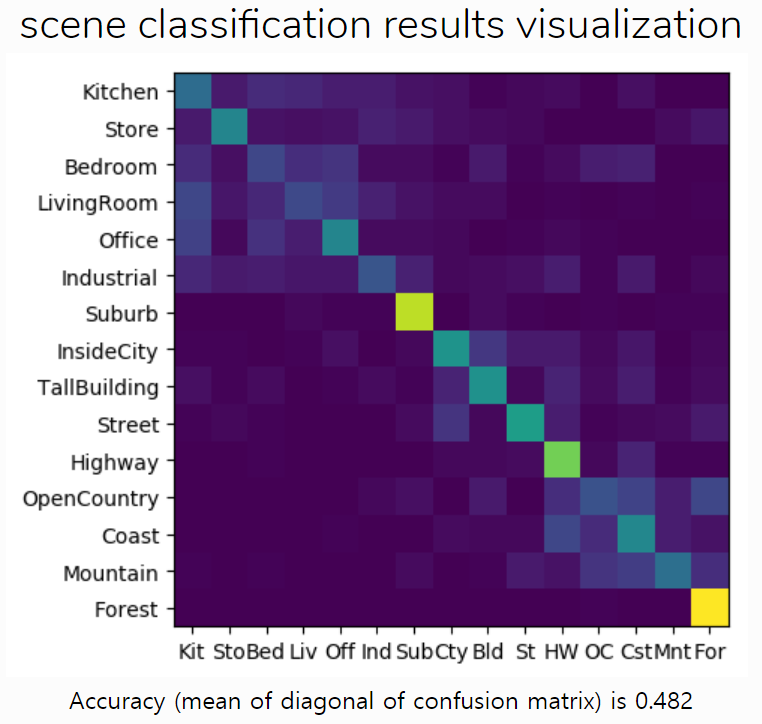
\includegraphics[width=8cm]{confusift.png}
    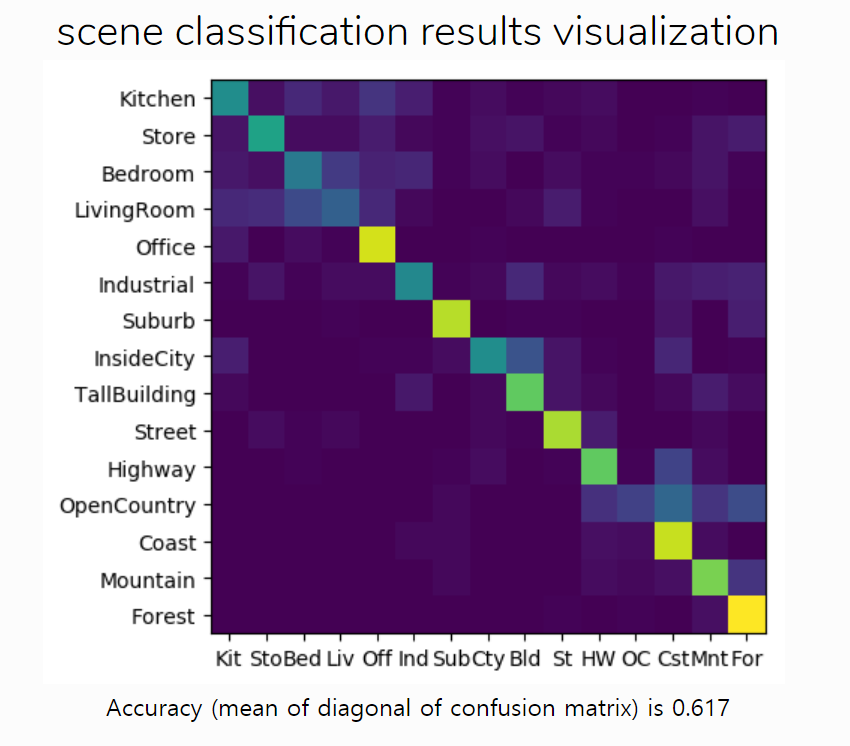
\includegraphics[width=8cm]{confulinear.png}
    \caption{\emph{Up:} Confusion matrix with SIFT features. \emph{Down:} Confusion matrix with HOG features. (In the both cases, I fixed the spatial pyramid representation and the linear kernel)}
    \label{fig:result1}
\end{figure}

HOG uses edge direction information, so it is suitable for identifying objects with unique outline,edge information, and SIFT can be matched irrespective of shape change, size change, rotation and so on because it is matched by the feature point unit of the model, so SIFT is a suitable method when the internal pattern is complicated , so the feature points are abundant. These results show that this data set is more robust to the HOG feature.

\pagebreak
\section*{Plots which visualizes PCA of the vocabulary}
\begin{figure}[h]
    \centering
    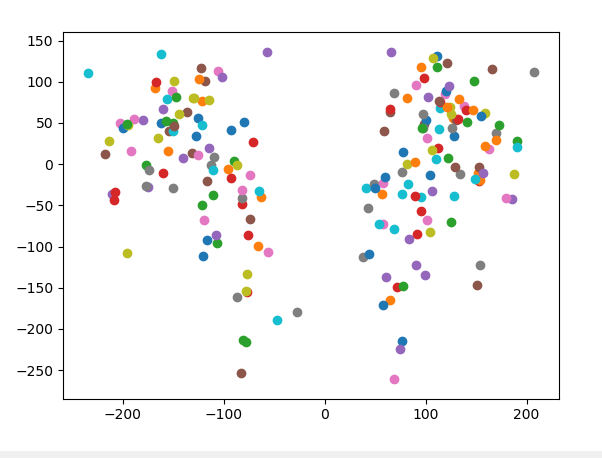
\includegraphics[width=10cm]{pca1.png}
    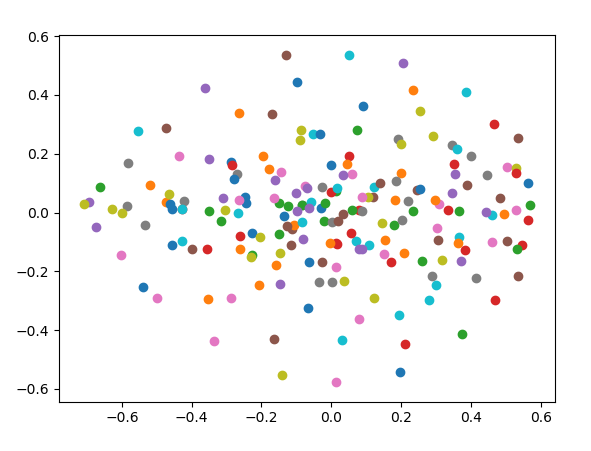
\includegraphics[width=10cm]{pca2.png}
    \caption{\emph{Up:} PCA of SIFT vocabulary. \emph{Down:} PCA of HOG vocabulary.}
    \label{fig:result1}
\end{figure}

As the distribution of principal components of codevectors spreads over the PCA graph, the codebook describes the more generalized features, so the HOG feature is better suited for this dataset. This result is the same as the results on the previous page.

\pagebreak
\section*{Recognition accuracy comparison between SVM kernels(linear vs. RBF)}
\begin{figure}[h]
    \centering
    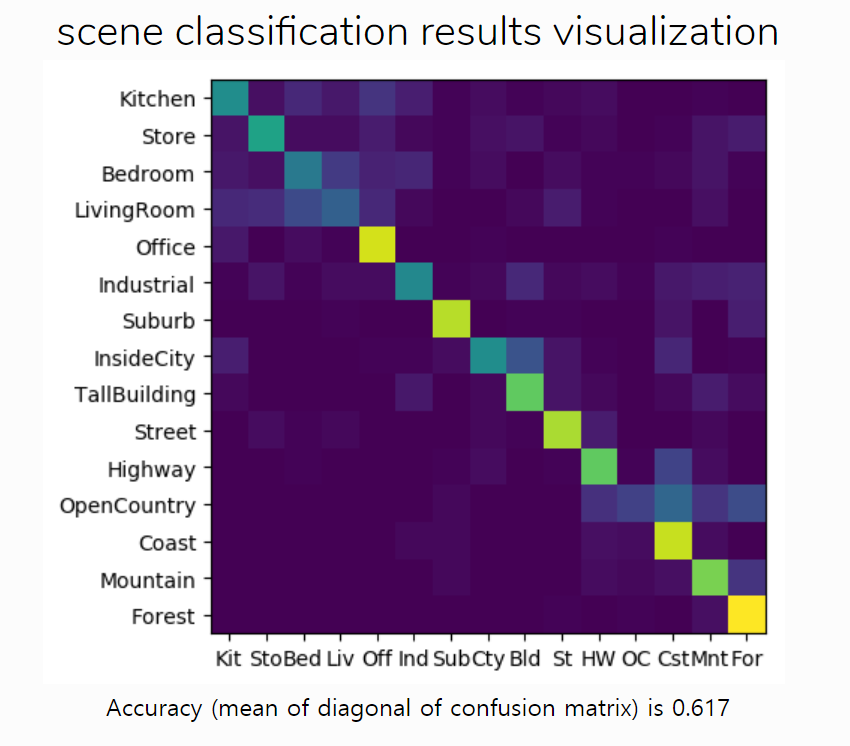
\includegraphics[width=8cm]{confulinear.png}
    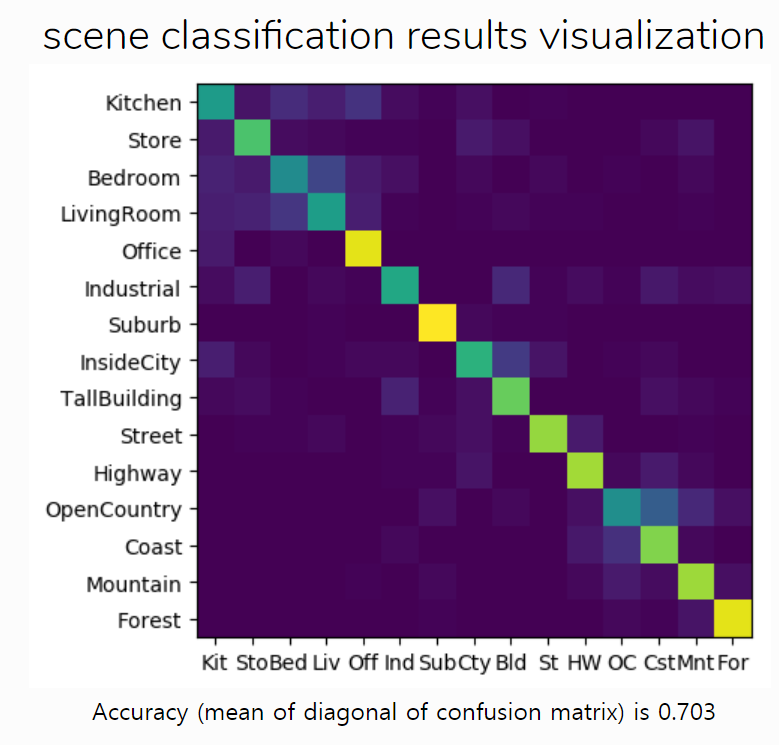
\includegraphics[width=8cm]{confubest.png}
    \caption{\emph{Up:} Confusion matrix with linear kernel. \emph{Down:} Confusion matrix with RBF. (In the both cases, I fixed the HOG feature and the spatial pyramid representation)}
    \label{fig:result1}
\end{figure}

It can be seen that the higher accuracy is obtained when mapping the data to the higher dimensional using RBF. Therefore, it can not be said that the linear separability of feature is strong at present without kernel trick.

\pagebreak
\section*{Recognition accuracy comparison between bag of words representation without spatial pyramid and that with spatial pyramid}
\begin{figure}[h]
    \centering
    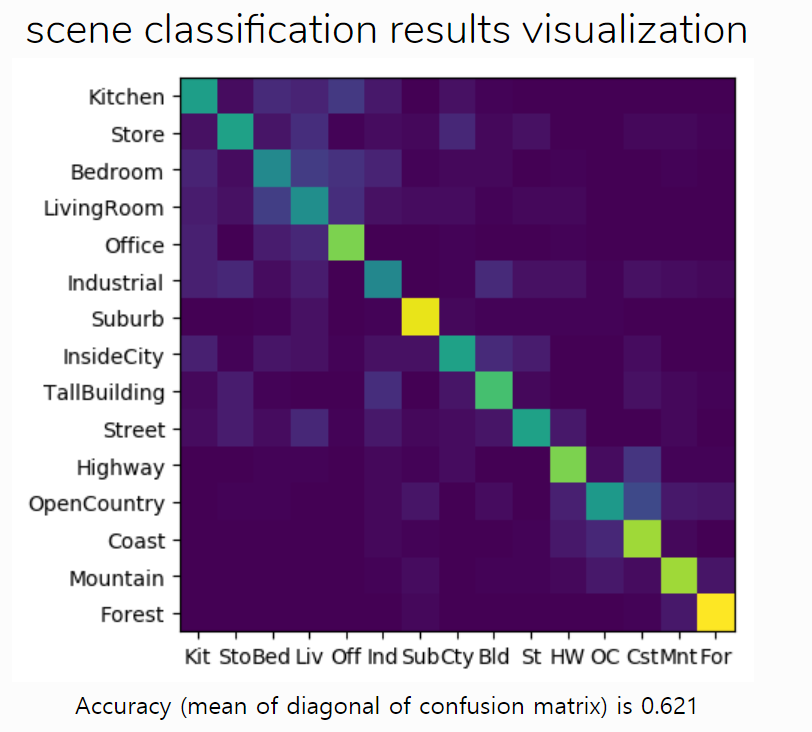
\includegraphics[width=8cm]{confubow.png}
    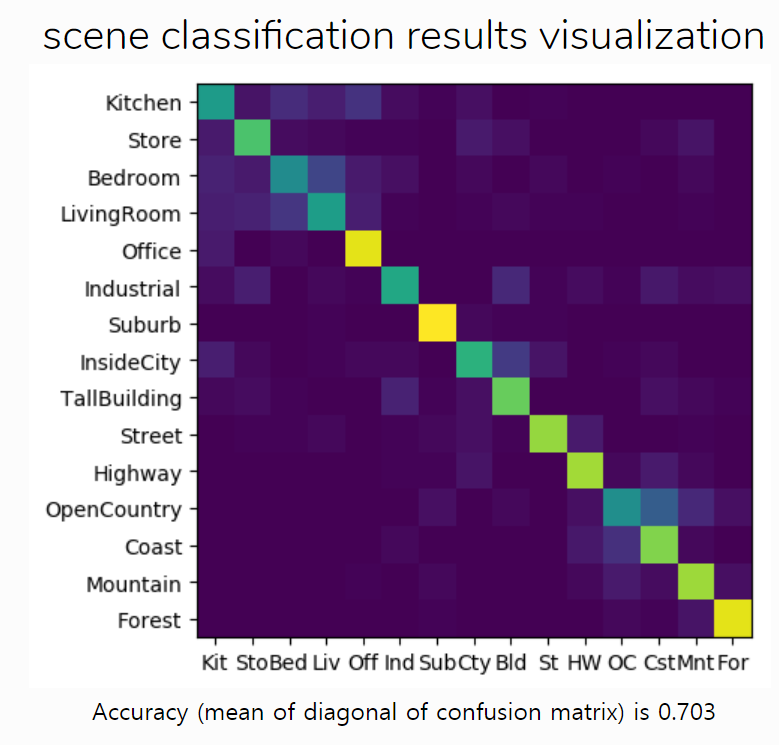
\includegraphics[width=8cm]{confubest.png}
    \caption{\emph{Up:} Confusion matrix without spatial pyramid. \emph{Down:} Confusion matrix with spatial pyramid. (In the both cases, I fixed the HOG feature and the RBF kernel)}
    \label{fig:result1}
\end{figure}

When using spatial pyramid representation, it takes more time than just using bag of words without spatial pyramid, but it can improve the accuracy by recovering some lost spatial information

\end{document} 